<<<<<<< HEAD

% This is LLNCS.DEM the demonstration file of
% the LaTeX macro package from Springer-Verlag
% for Lecture Notes in Computer Science,
% version 2.4 for LaTeX2e as of 16. April 2010
%
\documentclass[english]{llncs}
%
\usepackage{makeidx}  % allows for indexgeneration
%\usepackage{graphicx} % so we can include images
\usepackage[pdftex]{graphicx} % so we can include images
\usepackage[utf8]{inputenc} % display all characters properly
\usepackage[polish,danish,american,english]{babel}
\usepackage[T1]{fontenc}

\usepackage{url}
\usepackage{listingsutf8} % for listing code
\usepackage{color} % colors are nice

\definecolor{black}{rgb}{0,0,0}
\definecolor{gray}{rgb}{0.6,0.6,0.6}
\definecolor{white}{rgb}{1,1,1}

\definecolor{keywords}{rgb}{0.5,0,0.6}
\definecolor{strings}{rgb}{0,0.4,0}
\definecolor{comments}{rgb}{0.5,0.5,0.5}

\newcommand{\comment}[1]{}
\definecolor{Orange}{rgb}{1,0.5,0}
\newcommand{\todo}[1]{\textsf{\textbf{\textcolor{red}{[#1]}}}}

\lstset{language=Java,
  basicstyle=\ttfamily\footnotesize,
  numbers=left,
  numberstyle=\tiny\color{gray},
  stepnumber=1,
  numbersep=5pt,
  frame=single,
  tabsize=2,
  captionpos=b,
  breaklines=true,
  breakatwhitespace=true,
  keywordstyle=\color{keywords},
  commentstyle=\color{comments},
  stringstyle=\color{strings},
  extendedchars=true,
  inputencoding=utf8/latin1,
  texcl=true
}

%
\begin{document}
%
\frontmatter          % for the preliminaries
%o
\pagestyle{headings}  % switches on printing of running heads
\addtocmark{Code Generation From ECDAR} % additional mark in the TOC
%
\mainmatter              % start of the contributions
%
\title{Code Generation From ECDAR}
%
\titlerunning{Code Generation From ECDAR}  % abbreviated title (for running head)
%                                     also used for the TOC unless
%                                     \toctitle is used
%
\author{Rasmus Berntsen \and Florian Biermann \and Lauge Groes \and Nicolas Wainach Lundqvist Jensen \and Thomas Kokholm \and Piort Stawiski \and Wiktor Michal Zdziechowski}

\authorrunning{Rasmus Berntsen et al.} % abbreviated author list (for running head)

%%%% list of authors for the TOC (use if author list has to be modified)
\tocauthor{Rasmus Berntsen, Florian Biermann, Lauge Groes, Nicolas Wainach Lundqvist Jensen, Thomas Kokholm, Piort Stawiski, Wiktor Michal Zdziechowski}

\institute{IT University of Copenhagen, Denmark\\
\email{\{raber, fbier, lgro, nicl, tkok, psta, wmic\}@itu.dk}
}
\maketitle % typeset the title of the contribution

\begin{abstract}
This paper present a framework for code generation, based on timed automata modelled in ECDAR (Environment for Compositional Design and Analysis of Real Time Systems). A graphical tool based on UPPAAL that allows to visually create models of real-time systems.

The motivation for doing this project is, that the current version of the ECDAR framework is lacking an important feature: The possibility to utilize models for code generation, as a way to develop software solutions based on visually represented models.

The general approach of this project is to solve this aforementioned challenge: Show how one can generate true code, in this case Java, from an ECDAR model (\ref{implementation}). This is done in two closely related parts. The first part is a framework build to macth the single parts of the ECDAR specification (\ref{implementation-framework}). The second part presents how to generate compileable code from an ECDAR model. The code basis of the generated code is from the framework(\ref{implementation-code-generation}). In order to solve these tasks, it was necessary to create the notation of tasks as an extension to the ECDAR model, within the framework (\ref{subsec:tasks}). 

The functionality of the framework is evaluated through a series of test (\ref{Testing}). All of which is based on beverage-serving machine model (See figure \ref{bev-machine} on page \pageref{bev-machine}).

From our findings in the evaluation (\ref{evaluation}) \todo{Finish it when we have the evalulation in place}

\end{abstract}


\section{Introduction}
\label{introduction}
In the preceding years a new level of abstraction in development have been
evolving. Utilizing a higher level of abstraction, than high-level programming
languages, we have Model Driven Development. This new paradigm is combining a
focus on automation and code generation, to enable a new way of black boxing
solutions within a multitude of specialists outside traditional programming
while securing platform independency.

In this paper, we will propose a new code generator for the ECDAR tool (see
Sec. \ref{introduction-ecdar}. Until now, there exists no such generator. We
will outline our approach in detail and also look at related work to this
topic. While there already exists a code generator for a tool very similar to
ECDAR. However, ECDAR includes some features which make it incompatible with
these generators. The code we generate is executable in a simulator environment
and serves as a starting point for developing an embedded system.

\subsection {Real Time Computing}
\label{introduction-rts}

Real-time computing is the study of hardware and software systems that must
satisfy explicit response-time constraints or risk severe consequences,
including failure. Timed systems are used in a wide range of domains including
communications, embedded systems, real-time and automated control.  They can be
easily found in our environment; one of simple examples is the airbag system in
a car.  The real-time constraint in this system is the reaction time between
crash sensors receiving input and the deployment of airbags. Among some of the
important characteristics of real-time systems we can distinguish extreme
reliability and safety as they are very often safety-critical.

\subsection{ECDAR}
\label{introduction-ecdar}

The ``Environment for Compositional Design and Analysis of Real Time Systems''
(ECDAR) - is a graphical tool based on UPPAAL TIGA
\cite{behrmann_uppaal-tiga:_2006} that allows to visually create models of
real-time systems. Unlike UPPAAL \cite{larsen_uppaal_1997}, it is implementing a
complete specification theory for real time systems
\cite{David:2010:TIA:1755952.1755967,conf/atva/DavidLLNW10}. In ECDAR,
components of the system are described as automatons extended with clocks (timed
automata), that can be combined to form larger comprehensive system
descriptions. Correct specification of composition is supported by well defined
compositional reasoning theory, consisting of operators like: parallel
composition, conjunction, satisfaction checking and refinement. On the top of
that, the tool allows for scalable verification of models by querying the
implementation with verification questions \cite{conf/atva/DavidLLNW10}.


\subsection{Project}
\label{introduction-problemfield}
This paper will follow an implementation of code generation from ECDAR to
Java. The proposed implementation of the ECDAR code generator is split up in two
parts. The first part is a framework of abstract classes, implementing in as
much detail as possible the single elements used in ECDAR specifications. The
second is the actual code generation. Our code generator generates sources which
inherit from the abstract framework to minimize the amount of code that needs
actually to be generated. The paper will also detail the different testing
issues and benefits of implementing code generation for ECDAR.


\section{Background}
\label{background}
% LAST UPDATE: 13.12.2012 % 


\subsection{Timed Input/Output Automata}
\label{background-tioa}

The "Timed Input/Output Automata" is a basic, mathematical specification
framework for description and analysis of real time systems.  In this framework,
system is represented by non-deterministic, possibly infinite-state, state
machine referred as “timed I/O automaton” (TIOA)
\cite{Kaynar:2006:TTI:1203437}. TIOA has been implemented as the modeling
language in ECDAR \cite{conf/atva/DavidLLNW10}.

\begin{figure}[t]
\label{simple-model}
\begin{centering}
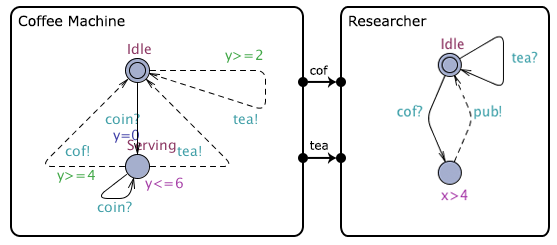
\includegraphics[scale=0.6]{images/simplefied_uni}
\par\end{centering}
\caption{Model of beverage-serving machine and researcher.}
\label{bev-machine}
\end{figure}

The preceding figure (see Fig. \ref{simple-model}) illustrates the system
consisting of two automatons: \emph{Coffee Machine} and \emph{Researcher}.  The
\emph{Coffee Machine}, given a coin (\emph{coin}), it serves either coffee
(\emph{cof}) or tea (\emph{tea}) to the \emph{Researcher} within a given time
interval. Moreover, free tea is served once in a while. The \emph{Researcher} is
producing publications (\emph{pub}), once provided a timely stimuli in form of
preferred beverage (\emph{cof}).  In the example, the \emph{Coffee Machine} -
TIOA consists of and two locations represented by circles: \emph{Idle} and
\emph{Serving}. \emph{Idle} represents the starting location, and the state of
machine waiting for coin input (\emph{coin?}). Analogously, the
\emph{Researcher} is in \emph{Idle} state expecting either coffee (\emph{cof})
or tea (\emph{tea}) provided by \emph{Coffee Machine}.  The flow of each TIOA is
controlled by three types of labels: \emph{invariants}, \emph{guards} and
\emph{clock-reset operations}.  Invariants are defined on locations ($y\leq 6$
and $x\textgreater 4$) and represent constraints for the clocks in order for the
control to remain in particular location until time requirement is fulfilled.
Guards are located on the edges ($y\geq 2$ and $y\geq 4$) and express conditions
on the values of clock that must be satisfied in order for the edge to be
taken. When the condition is satisfied, the transition occurs and action
(\emph{cof!}, \emph{tea!} or \emph{pub!}) is triggered. Clock-reset operations
($y=0$) are simple clock value manipulations in form of assignment that enforce
progress in the system.

In ECDAR, the specification interface is leveraging the UPPAAL TIGA language
\cite{behrmann_uppaal-tiga:_2006} to describe TIOA. However, the following
constraints are retained\footnote{See
  \url{http://people.cs.aau.dk/adavid/ecdar/examples.html#lang}}:


\begin{itemize}
\item Invariants may not be strict.
\item Inputs must use controllable edges.
\item Outputs must use uncontrollable edges.
\item All channels must be declared broadcast.
\item The system is implicitly input enabled due to broadcast communication but
  for refinement checking purposes the relevant inputs must be explicit in the
  model.
\item In the case of parallel composition of several components, a given output
  must be exclusive to one component.
\item For implementations, outputs must be urgent.
\item For implementations, every state must have independent time progress,
  i.e., progress must be ensured by either an output or infinite delay.
\item $\tau$-transitions (no output or input) are forbidden.
\item Global variables are forbidden.
\end{itemize}

\subsection{Code Generation}
\label{background-codegeneration}

In order to clarify what code generation is one need to understand what a model
transformation is, as this is a fundamental part of code generation. In short
one could say that the model transformation is a way to ensure that the final
code is consistent and with a reduced number of errors. The generation is an
automated way to produce code from models. The actual generation is defined by
the software developer, thus it is defined what the output should be, but the
input and the data is not.

There is generally two ways to do model transformations, that is model to model
and model to text, the former known as M2M and the latter M2T. There are also a
lot of other tools and techniques for transformation, which should not be
confused with model transformations. One could mention an XSLT-transformation as
an example, where the base input is an XML-document and the final output is
another XML-document, often XHTML, with a predefined XML-Schema.

Model to model is a transformation of a number of models to a given number of
new models -- from X number of models to Z number of new models. Model to text is
the transformation of a number of models to text, the text could for instance be
code -- which is why the process sometimes is known as model to code.



\section{Implementation}
\label{implementation}
The proposed implementation of the ECDAR code generator is split up
in two parts. The first part is a framework of abstract classes, implementing
in as much detail as possible the single parts of ECDAR specifications
(i.e. edges, locations, TIOA). The second is the actual code generation.
Our code generator generates sources which inherit from the abstract
framework to minimize the amount of code that needs actually to be
generated. This means that nearly all design decisions have been made
prior to generating code, reducing space for possible errors. This
section describes our implemented subset of ECDAR and the code generator
in detail.

\subsection{Tasks}

ECDAR defines the behavior of a system as a state machine. This behavior
is, however, still too abstract to justify code generation. We can
generate code which implements the behavior of state machines, but
in essence, the system would then only produce messages.

To make this tool more useful, we introduce the notion of tasks as
an extension to the language. Let $T_{S}$ be a set of tasks and $L_{S}$
a set of locations on a system $S$. Then $\forall l\in L_{s}\exists t\in T_{s}$,
i.e. each location is assigned exactly one task. A task is a procedure
which will be executed as soon as an automaton traverses over an edge,
arriving at a new location.

Tasks can either be preemptive or non-preemptive. This property becomes
important for defining behavior of automata when they are notified
about input by the controller.

ECDAR is input-enabled (see Sect. \ref{background-ecdar}) and therefore,
the system is required to react to input immediately. As a consequence,
there must also be a well defined reaction to input during the execution
of a task.

When an automaton is executing a task and it receives an input message
which it accepts, it may stop the currently executed task and proceed
as originally defined in ECDAR (i.e. traverse the corresponding edge),
if and only if the task is preemptive. Otherwise, the given input
will be ignored and the execution of the task continues.

To determine if a task is preemptive is up to the designer of the
system to decide. By default are all tasks non-preemptive.

\subsection{The ECDAR Framework}
\label{implementation-framework}

\begin{figure}[t]
\begin{centering}
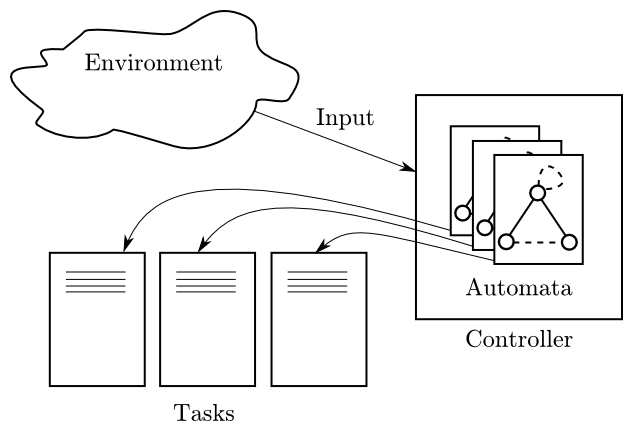
\includegraphics[scale=0.5]{images/ecdar_architecture} 
\par\end{centering}

\caption{Schematic of the architecture of our ECDAR implementation.}
\end{figure}

The architecture we chose is based upon the work of Amnell et al.\cite{amnell_code_2002}
with some modifications. Communication between automata is implemented
as message passing between environment and automata, where automata
send messages to the environment by traversing over output edges --
there are no shared variables (see Sect. \ref{background-tioa}). Messages
are processed by a controller object, which initializes automata and
also notifies automata about received messages.

We require multiple automata to execute in quasi-parallel. Therefore,
we do not queue tasks. Since the automata are moved to classical threading
architecture, we do not require multiple processor units. Instead,
the controller and each automaton run in separate threads. Since there
is no communication between automata directly, we can minimize synchronizing
so that nearly no waiting is required.

The following overview will give further implementation details on each
component of ECDAR as we implemented it. Each component is illustrated with a
short code example, implementing ECDAR's "University"
example \footnote{\url{http://people.cs.aau.dk/adavid/ecdar/examples.html\#university}}. For
clarity, we omit the framework implementation and focus on the generated code.

\subsubsection{Locations.}

Each location is a associated with a task. Task execution is implemented
in a separate thread, not blocking the execution of the automaton.
Locations are implemented as objects holding an array of edges that
point away from it. (See Fig. \ref{location-example})

\begin{figure}[t]
\lstinputlisting[linerange={101-132}]{code/Machine.java}
\caption{Example of location code.}
\label{location-example}
\end{figure}


\subsubsection{Edges.}

An edge holds a reference to the location which the parent automaton
will be at after traversing this very edge. Edges can be asked if
they will be available at a given time. This is implemented to enable
lazy waiting in the automaton's traversal checker. Each edge is associated
with some input. If an edge is controllable, it will be triggered
if the automaton is notified at this input. If it is uncontrollable,
it will send its input to the controller. Furthermore, edges have
access to the clock of the parent automaton to reset it appropriately.

The implementation makes a class-wise distinction between controllable
and uncontrollable edges and hard-codes the behavior for given input.
Such hard-coded features are e.g. notifying the controller on traversing
an uncontrollable edge. (See Fig. \ref{edge-example})


\subsection{TIOA.}

The implementation of timed I/O automata holds a set of locations
and a reference to the location it is currently at. The TIOA is executed
by a thread that keeps checking for available edges and traverses
along these, as soon as they become enabled. To check if an edge is
available, let $E_{s\rightarrow t}$ be an edge where $s,\, t$ are
start and target locations respectively. Furthermore, let $g(E)$
be a function evaluating the guard of an edge $E$ and $I(l)$ a function
evaluating the invariant of a location $l$. Our implementation uses
$g'(E_{s\rightarrow t})=g(E_{s\rightarrow t})\wedge I(t)$ to check
if $E_{s\rightarrow t}$ is available.

Additionally, the automaton has the ability to return the current
local clock state (see \ref{implementation-presumptions}) and to
reset the clock. We use the same notion of clocks as \cite{amnell_code_2002},
where time on the local clock is the difference between the current
time on the system clock and the time the local clock was started.
Resetting the local clock means to use the current system clock time
as the new start time. (See Fig. \ref{tioa-example})

\begin{figure}[t]
\lstinputlisting[linerange={8-8,169-184}]{code/Machine.java}
\caption{Example of TIOA code.}
\label{tioa-example}
\end{figure}


\subsubsection{Controller.}

The controller holds all automata given in the specification, executes
them initially in quasi-parallel and notifies automata about input
from the environment. It is a singleton, accessible in a static fashion.
This property is useful for uncontrollable edges that need to notify
the controller about input. (See Fig. \ref{controller-example})

\begin{figure}[t]
\lstinputlisting[linerange={6-11,63-64}]{code/UniversityController.java}
\caption{Example of controller code.}
\label{controller-example}
\end{figure}


\subsection{Synchronization}

In the framework implementation, the Java keyword \textit{synchronized} is 
used for making certain operations quasi-atomic. That means, that a set of
instructions may not be interrupted by the execution of another thread -- 
i.e. traversals over edges.

This is mainly used for the logging of signals, so that logging time
is preserved and the output appears in the right order. \textit{Synchronized}
is also used, to set some internal states on TIOA, where the internal state
consists of multiple values that need to be set at the same time.

\textit{Synchronized} is furthermore used to prioritize handling of input.  The
method on the controller object, that is handling the signal, as well as those
on the TIOA that react to a signal if it is accepted, are modified with
\textit{synchronized}. This ensures that, before everything else, the input is
processed.


\subsection{Code Generation}
\label{implementation-code-generation}

In the implementation presented the actual generation of source code is done
through a model to text transformation. The generation outputs compilable
JAVA-code based on input from an ECDAR file.

The Eclipse Modeling Framework (EMF) is utilized for the process. EMF is a
modeling framework and code generation facility for building applications based
on a structured data model. From a model specification described in XMI, EMF
provides tools and runtime support to produce a set of Java classes for the
model, along with a set of adapter classes that enable viewing and command-based
editing of the model and it provides a basic editor.  The core EMF framework
includes a meta model (Ecore) for describing models and runtime support for the
models including: change notification, persistence support with default XMI
serialization, and a very efficient reflective API for manipulating EMF objects
generically. In the implementation presented in this paper an Xtext environment
is generated from the ECDAR Ecore model. Xtext is a framework for development of
programming languages and domain specific languages.

In order to generate code from the model it's imperative to follow a process of
multiple steps: Get the input from ECDAR, translate this to Xtext ECDAR DSL,
setup a workflow that manages the process and finally a XPAND-template is needed
to define how the transformation output should look like. Each step is being
described in more detail in the following section.

\subsubsection{Transformation process}
\label{transformation-process}

The initial output from the ECDAR tool is in the XML-format. This XML-output
contains a complete definition of the model with locations, edges, variables,
transformations etc. In order to work with these files and do the actual code
generation, a conversion to Xtext ECDAR DSL is needed. For this conversion we
are using a converter (courtesy of Bastian) that simply takes the ECDAR XML-file
and converts it to ECDAR DSL. The ECDAR DSL syntax is defined in our Xtext ECDAR
environment. With the combination of the Ecore meta model and the Xtext syntax a
workflow can be defined. This workflow is describing how to handle the
generation process. This is done with the help of the Modeling Workflow Engine 2
(MWE2). Also referenced in the workflow is the template that describes how the
actual output is going to look like. The templates are written using
Xpand. Xpand is a statically typed template language. Conveniently Xpand
supports code-completion directly connected to the Ecore model defined in the
MWE2 workflow, but also comes with syntax coloring, refactoring and error
highlighting. The output generation results for the system presented in this
paper are based on serveral workflows and templates to do the rather complex
transformations: One set of workflows and templates for respectively the
Specification, Controller and Environment.

More specifically in the workflow-file one defines what model to use, a
slot-name to refer to later and an entry point. The entry point defines which
class element is the top or root element. The entry-element that is defined for
the three afformentioned workflows is "ETSpecificationDefinition". Also defined
in the workflow is how to use the entry-element. For instance in the
specification workflow it is defined that for each "ETSpecificationDefinition" a
transformation is done using the Xpand template for this particular
generation. The end result is having generated ouput for each specification that
was initialy described and modeled from within the ECDAR XML-file.

With the workflow fully configured, the next step is to write the
transformation. This is done in a Xpand template. The snippets in figure
\ref{xpand-example} shows some important steps.

\begin{figure}[t]
\lstinputlisting[linerange={1-2}]{code/TemplateSpecifications.xpt}
\lstinputlisting[linerange={6-6}]{code/TemplateSpecifications.xpt}
\lstinputlisting[linerange={34-41}]{code/TemplateSpecifications.xpt}
\caption{Snippets from Xpand-template \label{xpand-example}}
\end{figure}

The arrows, known as guillemets (``\guillemotleft'' and `` \guillemotright''),
shows where in figure \ref{xpand-example} the XPAND language is in place. First
of all an import of the model is done in the first line, referenced as
ecdarText. We then proceed to one of the central concepts of Xpand by using the
define-block; This is where we define our template. We only use one template is
this specific file, but it could have contained multiple, which would have
resulted in multiple define-blocks. In the next and last snippet we jump to a
part where we are iterating through each edge and create a constructor for the
current class. In the first line we create the constructor by inserting the text
"Edge" and add the number the iterator has reached. We then iterate through a
list of the current Edges variables, which should be one signal, and returns the
results as a list. We furthermore use a new iterator to keep track of this
itereation. We afterwards check if it's the first iteration, and if it is, we
print out the edges target name and the variable signal, such as "super(C,
"signal");".

The notion of tasks as previous described in section 3.2. is accounted for in
our generated output. In the controller we generate functions that will be
invoked at each location. A task is a procedure which will be executed as soon
as an automaton traverses over an edge, arriving at a new location. There can
only be one task pr. location. The thought behind having all methods in the
controller is for a better overview and a centralized customizeable file.



\section{Evaluation and Discussion}
\label{evaluation}
\subsection{Testing}
\label{Testing}
In order to test our software solution three different testing methods have been
arranged.

\subsubsection{Compiling properly}
Making sure every output compiles properly.

\subsubsection{Log file testing}
For this project a log file analysis program have been incorporated. A small
program verifying that the signals in the generator code are fired in the right
order according to the input model.  The analysis program is hard coded to match
our testing model (see Fig. \ref{simple-model}). Thus it is checking for signals
like: GRANT, COIN and TEA, in the specified order. If a signal is called within
the generator before it is supposed too (e.g TEA before COIN) the analysis
program will call for an ERROR.

The log file contain time stamps of global time from each automaton in a model. The
global time can then be verified by comparison with time assigned within the
ECDAR modelling tool.

\subsubsection{Manual Comparison}
Final testing procedure is a manual step-by-step comparison of a simple
graphical automaton model and the corresponding code generated. Cycling through
the times, comparing each step with the output.
%(verified by Andrzej Wasowski).

\subsection{Presumptions and Resulting Motivations}
\label{implementation-presumptions}

Our implementation represents only a subset of actual ECDAR. Currently, the
implementation assumes only one clock per automaton. Also, we assume the
specification to be valid, since there are other tools that verify
correctness\footnote{\url{http://people.cs.aau.dk/adavid/ecdar/}}.

The only operator we implement for code generation is the parallel
composition operator. Let $M$ be the type ECDAR specification. Then
all operators in ECDAR are of type $M_{i}\otimes M_{j}\rightarrow M_{ij}$.
Other than for the majority of operators, which refine the specification,
it is impractical to implement parallel composition as a model-to-model
transformation, since it produces the cross-product of two models
\cite{david_compositional_2012}. These models are size $|M_{i}|\cdot|M_{j}|$
and generating code for them would consume a large amount of memory
and raise complexity. This would be inappropriate for an embedded
system. We elaborate on this further in Sect. \ref{implementation-framework}.

ECDAR specifications are written on the assumption of the synchrony
hypothesis (see Sect. \ref{background-ecdar}) \cite{david_compositional_2012}.
This is an important property for code generation, as reasoning about
time differences in execution becomes unnecessary for the developer.
However, we still kept overhead low to achieve reasonable fast performance.

%To produce feasible code that would be able to run on embedded systems,
%we targeted Real-Time Java (Java RTS)%
%\footnote{\href{}{http://www.oracle.com/technetwork/java/javase/tech/index-jsp-139921.html}%
%}. Java RTS was designed to improve upon standard Java in terms of
%timing accuracy an real-time embedded systems.





\section{Related Work}
\label{related}
The aim of this project is to develop a tool for automatic synthesis of Java-code, from the modelling tool: ECDAR. However there already exist tools similar too ECDAR.

TIMES\footnote{\url{http://www.timestool.com}}: is a graphical tool set for modelling, schedulability analysis for implementation of embedded systems. It allows users to model a system and the abstract behaviour of its environment. 
Like ECDAR, TIMES is based on timed automata (See section \ref{introduction-ecdar} on page \pageref{introduction-ecdar} for more details on automaton). Similarly TIMES derive from UPPAAL and is based on the standard for modelling real-time systems \cite{Alur1994:183}.
Times is extended by real-time tasks, checking the reachability and schedulability of a modelled automata. It too can simulate models and validate dynamic behaviour of a system: Users can see how tasks executes according to time. The simulator shows a graphical representation of the generated trace, showing the time points when the tasks are released, invoked, suspended, resumed, and completed.

TIMES can be used for code-generate, as illustrated Tobias Amnell et al \cite{Amnell:2002:CST:779110.779112}. They generate C-code for a Lego Mindstorms system using TIMES, checking for reachability and schedulability. Simulor to what we trying to do with ECDAR. 

%----
There are certain differences between TIMES and ECDAR, despite the missing feature of code generation in ECDAR. In contrast to TIMES's programmable logic controllers, a scheduling approach is not suf?cient to deal with unpredictable behaviour in ECDAR.
Looking at what are taking as input by the controller - TIMES simple takes a model, checking reachability and schedulability, whereas ECDAR synthesise each component in a model.



\paragraph{Composable Code Generation for Model-Based Development}
by Kirk Schloegel et al. present a framework for generating
code\cite{composable-code-generation}. They emphasize how utilizing their
framework, code generators aren't programs separated from a corresponding
graphical model as it often have been in the past. Our code generator isn't
based on this framework, however their approach on developing code generators
with focus on graphical models is related to our approach with ECDAR.

\paragraph{Code Synthesis for Timed Automata}
by Tobias Amnell et al. present a framework for the development of real-time
embedded systems\cite{Amnell:2002:CST:779110.779112}. Their work is similar to
our project. In the article the illustrate how their framework is based on timed
automata and real-time tasks - relative to our concept with ECDAR.




\section{Conclusion}
\label{conclusion}
In this project we showed a valid approach towards developing a code 
generator for TIOA models created by ECDAR. 

First by building a framework of abstract classes in Java, based on 
ECDAR. This entails locations, edges and TIOA with a modified messaging 
system based on tasks and a controller class. The Java keyword 
\textit{synchronized} is used for logging time, internal states and 
maintaining priority. 

Secondly by defining the code generation, with a model to text 
transformation, that inherits from the abstract classes in the 
framework. More concretely used the translated input from ECDAR, and 
utilized an Xpand-template to generate the code. 

In our implementation we assumed ECDAR specifications to be valid. 
Testing was accomplished through compiling, automatic and manual log 
file testing. 

Further work is possible by converting our framework for use with the 
Real-Time Specification for Java (RTSJ). RTSJ is a set of interfaces and 
behavioral specifications that allow for real-time programming in the 
Java programming language 
\footnote{\url{http://www.oracle.com/technetwork/java/javase/tech/index- 
jsp-139921.html}}. So ``real-time'' is about predictable timing. In our 
implementation we don't utilize RTSJ, so we can't currently guarantee 
thread prioritization and timing. 



\section{Acknowledgements}
\label{acknowledgements}
The XML to Xtext ECDAR DSL, as mentioned in section~\ref{transformation-process} on page~\pageref{transformation-process}, is developed by Bastian M\"uller, student at IT Unviversity of Copenhagen.

The project has been carried out with supervision from Andrzej Wasowski,
Associate Professor at IT University of Copenhagen.

All source code we used and produced over the course of this project can be found
at \url{https://github.com/tkok/MDD-E2012-P6}.


\bibliographystyle{plain}
\nocite{*}
\bibliography{MDD}

\appendix
\section{First Appendix}

\end{document}
=======

% This is LLNCS.DEM the demonstration file of
% the LaTeX macro package from Springer-Verlag
% for Lecture Notes in Computer Science,
% version 2.4 for LaTeX2e as of 16. April 2010
%
\documentclass[english]{llncs}
%
\usepackage{makeidx}  % allows for indexgeneration
%\usepackage{graphicx} % so we can include images
\usepackage[pdftex]{graphicx} % so we can include images
\usepackage[utf8]{inputenc} % display all characters properly
\usepackage[polish,danish,american,english]{babel}
\usepackage[T1]{fontenc}

\usepackage{url}
\usepackage{listingsutf8} % for listing code
\usepackage{color} % colors are nice

\definecolor{black}{rgb}{0,0,0}
\definecolor{gray}{rgb}{0.6,0.6,0.6}
\definecolor{white}{rgb}{1,1,1}

\definecolor{keywords}{rgb}{0.5,0,0.6}
\definecolor{strings}{rgb}{0,0.4,0}
\definecolor{comments}{rgb}{0.5,0.5,0.5}

\newcommand{\comment}[1]{}
\definecolor{Orange}{rgb}{1,0.5,0}
\newcommand{\todo}[1]{\textsf{\textbf{\textcolor{Orange}{[#1]}}}}

\lstset{language=Java,
  basicstyle=\ttfamily\footnotesize,
  numbers=left,
  numberstyle=\tiny\color{gray},
  stepnumber=1,
  numbersep=5pt,
  frame=single,
  tabsize=2,
  captionpos=b,
  breaklines=true,
  breakatwhitespace=true,
  keywordstyle=\color{keywords},
  commentstyle=\color{comments},
  stringstyle=\color{strings},
  extendedchars=true,
  inputencoding=utf8/latin1,
  texcl=true
}

%
\begin{document}
%
\frontmatter          % for the preliminaries
%o
\pagestyle{headings}  % switches on printing of running heads
\addtocmark{Code Generation From ECDAR} % additional mark in the TOC
%
\mainmatter              % start of the contributions
%
\title{Code Generation From ECDAR}
%
\titlerunning{Code Generation From ECDAR}  % abbreviated title (for running head)
%                                     also used for the TOC unless
%                                     \toctitle is used
%
\author{Rasmus Berntsen \and Florian Biermann \and Lauge Groes \and Nicolas Wainach Lundqvist Jensen \and Thomas Kokholm \and Piort Stawiski \and Wiktor Michal Zdziechowski}

\authorrunning{Rasmus Berntsen et al.} % abbreviated author list (for running head)

%%%% list of authors for the TOC (use if author list has to be modified)
\tocauthor{Rasmus Berntsen, Florian Biermann, Lauge Groes, Nicolas Wainach Lundqvist Jensen, Thomas Kokholm, Piort Stawiski, Wiktor Michal Zdziechowski}

\institute{IT University of Copenhagen, Denmark\\
\email{\{raber, fbier, lgro, nicl, tkok, psta, wmic\}@itu.dk}
}
\maketitle % typeset the title of the contribution

\begin{abstract}
This paper present a framework for code generation, based on timed automata modelled in ECDAR (Environment for Compositional Design and Analysis of Real Time Systems). A graphical tool based on UPPAAL that allows to visually create models of real-time systems.

The motivation for doing this project is, that the current version of the ECDAR framework is lacking an important feature: The possibility to utilize models for code generation, as a way to develop software solutions based on visually represented models.

The general approach of this project is to solve this aforementioned challenge: Show how one can generate true code, in this case Java, from an ECDAR model (\ref{implementation}). This is done in two closely related parts. The first part is a framework build to macth the single parts of the ECDAR specification (\ref{implementation-framework}). The second part presents how to generate compileable code from an ECDAR model. The code basis of the generated code is from the framework(\ref{implementation-code-generation}). In order to solve these tasks, it was necessary to create the notation of tasks as an extension to the ECDAR model, within the framework (\ref{subsec:tasks}). 

The functionality of the framework is evaluated through a series of test (\ref{Testing}). All of which is based on beverage-serving machine model (See figure \ref{bev-machine} on page \pageref{bev-machine}).

From our findings in the evaluation (\ref{evaluation}) \todo{Finish it when we have the evalulation in place}

\end{abstract}


\section{Introduction}
\label{introduction}
In the preceding years a new level of abstraction in development have been
evolving. Utilizing a higher level of abstraction, than high-level programming
languages, we have Model Driven Development. This new paradigm is combining a
focus on automation and code generation, to enable a new way of black boxing
solutions within a multitude of specialists outside traditional programming
while securing platform independency.

In this paper, we will propose a new code generator for the ECDAR tool (see
Sec. \ref{introduction-ecdar}. Until now, there exists no such generator. We
will outline our approach in detail and also look at related work to this
topic. While there already exists a code generator for a tool very similar to
ECDAR. However, ECDAR includes some features which make it incompatible with
these generators. The code we generate is executable in a simulator environment
and serves as a starting point for developing an embedded system.

\subsection {Real Time Computing}
\label{introduction-rts}

Real-time computing is the study of hardware and software systems that must
satisfy explicit response-time constraints or risk severe consequences,
including failure. Timed systems are used in a wide range of domains including
communications, embedded systems, real-time and automated control.  They can be
easily found in our environment; one of simple examples is the airbag system in
a car.  The real-time constraint in this system is the reaction time between
crash sensors receiving input and the deployment of airbags. Among some of the
important characteristics of real-time systems we can distinguish extreme
reliability and safety as they are very often safety-critical.

\subsection{ECDAR}
\label{introduction-ecdar}

The ``Environment for Compositional Design and Analysis of Real Time Systems''
(ECDAR) - is a graphical tool based on UPPAAL TIGA
\cite{behrmann_uppaal-tiga:_2006} that allows to visually create models of
real-time systems. Unlike UPPAAL \cite{larsen_uppaal_1997}, it is implementing a
complete specification theory for real time systems
\cite{David:2010:TIA:1755952.1755967,conf/atva/DavidLLNW10}. In ECDAR,
components of the system are described as automatons extended with clocks (timed
automata), that can be combined to form larger comprehensive system
descriptions. Correct specification of composition is supported by well defined
compositional reasoning theory, consisting of operators like: parallel
composition, conjunction, satisfaction checking and refinement. On the top of
that, the tool allows for scalable verification of models by querying the
implementation with verification questions \cite{conf/atva/DavidLLNW10}.


\subsection{Project}
\label{introduction-problemfield}
This paper will follow an implementation of code generation from ECDAR to
Java. The proposed implementation of the ECDAR code generator is split up in two
parts. The first part is a framework of abstract classes, implementing in as
much detail as possible the single elements used in ECDAR specifications. The
second is the actual code generation. Our code generator generates sources which
inherit from the abstract framework to minimize the amount of code that needs
actually to be generated. The paper will also detail the different testing
issues and benefits of implementing code generation for ECDAR.


\section{Background}
\label{background}
% LAST UPDATE: 13.12.2012 % 


\subsection{Timed Input/Output Automata}
\label{background-tioa}

The "Timed Input/Output Automata" is a basic, mathematical specification
framework for description and analysis of real time systems.  In this framework,
system is represented by non-deterministic, possibly infinite-state, state
machine referred as “timed I/O automaton” (TIOA)
\cite{Kaynar:2006:TTI:1203437}. TIOA has been implemented as the modeling
language in ECDAR \cite{conf/atva/DavidLLNW10}.

\begin{figure}[t]
\label{simple-model}
\begin{centering}
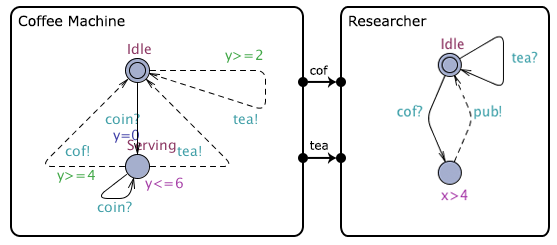
\includegraphics[scale=0.6]{images/simplefied_uni}
\par\end{centering}
\caption{Model of beverage-serving machine and researcher.}
\label{bev-machine}
\end{figure}

The preceding figure (see Fig. \ref{simple-model}) illustrates the system
consisting of two automatons: \emph{Coffee Machine} and \emph{Researcher}.  The
\emph{Coffee Machine}, given a coin (\emph{coin}), it serves either coffee
(\emph{cof}) or tea (\emph{tea}) to the \emph{Researcher} within a given time
interval. Moreover, free tea is served once in a while. The \emph{Researcher} is
producing publications (\emph{pub}), once provided a timely stimuli in form of
preferred beverage (\emph{cof}).  In the example, the \emph{Coffee Machine} -
TIOA consists of and two locations represented by circles: \emph{Idle} and
\emph{Serving}. \emph{Idle} represents the starting location, and the state of
machine waiting for coin input (\emph{coin?}). Analogously, the
\emph{Researcher} is in \emph{Idle} state expecting either coffee (\emph{cof})
or tea (\emph{tea}) provided by \emph{Coffee Machine}.  The flow of each TIOA is
controlled by three types of labels: \emph{invariants}, \emph{guards} and
\emph{clock-reset operations}.  Invariants are defined on locations ($y\leq 6$
and $x\textgreater 4$) and represent constraints for the clocks in order for the
control to remain in particular location until time requirement is fulfilled.
Guards are located on the edges ($y\geq 2$ and $y\geq 4$) and express conditions
on the values of clock that must be satisfied in order for the edge to be
taken. When the condition is satisfied, the transition occurs and action
(\emph{cof!}, \emph{tea!} or \emph{pub!}) is triggered. Clock-reset operations
($y=0$) are simple clock value manipulations in form of assignment that enforce
progress in the system.

In ECDAR, the specification interface is leveraging the UPPAAL TIGA language
\cite{behrmann_uppaal-tiga:_2006} to describe TIOA. However, the following
constraints are retained\footnote{See
  \url{http://people.cs.aau.dk/adavid/ecdar/examples.html#lang}}:


\begin{itemize}
\item Invariants may not be strict.
\item Inputs must use controllable edges.
\item Outputs must use uncontrollable edges.
\item All channels must be declared broadcast.
\item The system is implicitly input enabled due to broadcast communication but
  for refinement checking purposes the relevant inputs must be explicit in the
  model.
\item In the case of parallel composition of several components, a given output
  must be exclusive to one component.
\item For implementations, outputs must be urgent.
\item For implementations, every state must have independent time progress,
  i.e., progress must be ensured by either an output or infinite delay.
\item $\tau$-transitions (no output or input) are forbidden.
\item Global variables are forbidden.
\end{itemize}

\subsection{Code Generation}
\label{background-codegeneration}

In order to clarify what code generation is one need to understand what a model
transformation is, as this is a fundamental part of code generation. In short
one could say that the model transformation is a way to ensure that the final
code is consistent and with a reduced number of errors. The generation is an
automated way to produce code from models. The actual generation is defined by
the software developer, thus it is defined what the output should be, but the
input and the data is not.

There is generally two ways to do model transformations, that is model to model
and model to text, the former known as M2M and the latter M2T. There are also a
lot of other tools and techniques for transformation, which should not be
confused with model transformations. One could mention an XSLT-transformation as
an example, where the base input is an XML-document and the final output is
another XML-document, often XHTML, with a predefined XML-Schema.

Model to model is a transformation of a number of models to a given number of
new models -- from X number of models to Z number of new models. Model to text is
the transformation of a number of models to text, the text could for instance be
code -- which is why the process sometimes is known as model to code.



\section{Implementation}
\label{implementation}
The proposed implementation of the ECDAR code generator is split up
in two parts. The first part is a framework of abstract classes, implementing
in as much detail as possible the single parts of ECDAR specifications
(i.e. edges, locations, TIOA). The second is the actual code generation.
Our code generator generates sources which inherit from the abstract
framework to minimize the amount of code that needs actually to be
generated. This means that nearly all design decisions have been made
prior to generating code, reducing space for possible errors. This
section describes our implemented subset of ECDAR and the code generator
in detail.

\subsection{Tasks}

ECDAR defines the behavior of a system as a state machine. This behavior
is, however, still too abstract to justify code generation. We can
generate code which implements the behavior of state machines, but
in essence, the system would then only produce messages.

To make this tool more useful, we introduce the notion of tasks as
an extension to the language. Let $T_{S}$ be a set of tasks and $L_{S}$
a set of locations on a system $S$. Then $\forall l\in L_{s}\exists t\in T_{s}$,
i.e. each location is assigned exactly one task. A task is a procedure
which will be executed as soon as an automaton traverses over an edge,
arriving at a new location.

Tasks can either be preemptive or non-preemptive. This property becomes
important for defining behavior of automata when they are notified
about input by the controller.

ECDAR is input-enabled (see Sect. \ref{background-ecdar}) and therefore,
the system is required to react to input immediately. As a consequence,
there must also be a well defined reaction to input during the execution
of a task.

When an automaton is executing a task and it receives an input message
which it accepts, it may stop the currently executed task and proceed
as originally defined in ECDAR (i.e. traverse the corresponding edge),
if and only if the task is preemptive. Otherwise, the given input
will be ignored and the execution of the task continues.

To determine if a task is preemptive is up to the designer of the
system to decide. By default are all tasks non-preemptive.

\subsection{The ECDAR Framework}
\label{implementation-framework}

\begin{figure}[t]
\begin{centering}
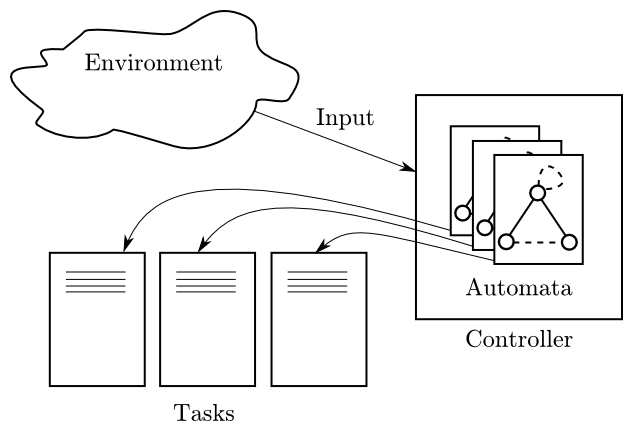
\includegraphics[scale=0.5]{images/ecdar_architecture} 
\par\end{centering}

\caption{Schematic of the architecture of our ECDAR implementation.}
\end{figure}

The architecture we chose is based upon the work of Amnell et al.\cite{amnell_code_2002}
with some modifications. Communication between automata is implemented
as message passing between environment and automata, where automata
send messages to the environment by traversing over output edges --
there are no shared variables (see Sect. \ref{background-tioa}). Messages
are processed by a controller object, which initializes automata and
also notifies automata about received messages.

We require multiple automata to execute in quasi-parallel. Therefore,
we do not queue tasks. Since the automata are moved to classical threading
architecture, we do not require multiple processor units. Instead,
the controller and each automaton run in separate threads. Since there
is no communication between automata directly, we can minimize synchronizing
so that nearly no waiting is required.

The following overview will give further implementation details on each
component of ECDAR as we implemented it. Each component is illustrated with a
short code example, implementing ECDAR's "University"
example \footnote{\url{http://people.cs.aau.dk/adavid/ecdar/examples.html\#university}}. For
clarity, we omit the framework implementation and focus on the generated code.

\subsubsection{Locations.}

Each location is a associated with a task. Task execution is implemented
in a separate thread, not blocking the execution of the automaton.
Locations are implemented as objects holding an array of edges that
point away from it. (See Fig. \ref{location-example})

\begin{figure}[t]
\lstinputlisting[linerange={101-132}]{code/Machine.java}
\caption{Example of location code.}
\label{location-example}
\end{figure}


\subsubsection{Edges.}

An edge holds a reference to the location which the parent automaton
will be at after traversing this very edge. Edges can be asked if
they will be available at a given time. This is implemented to enable
lazy waiting in the automaton's traversal checker. Each edge is associated
with some input. If an edge is controllable, it will be triggered
if the automaton is notified at this input. If it is uncontrollable,
it will send its input to the controller. Furthermore, edges have
access to the clock of the parent automaton to reset it appropriately.

The implementation makes a class-wise distinction between controllable
and uncontrollable edges and hard-codes the behavior for given input.
Such hard-coded features are e.g. notifying the controller on traversing
an uncontrollable edge. (See Fig. \ref{edge-example})


\subsection{TIOA.}

The implementation of timed I/O automata holds a set of locations
and a reference to the location it is currently at. The TIOA is executed
by a thread that keeps checking for available edges and traverses
along these, as soon as they become enabled. To check if an edge is
available, let $E_{s\rightarrow t}$ be an edge where $s,\, t$ are
start and target locations respectively. Furthermore, let $g(E)$
be a function evaluating the guard of an edge $E$ and $I(l)$ a function
evaluating the invariant of a location $l$. Our implementation uses
$g'(E_{s\rightarrow t})=g(E_{s\rightarrow t})\wedge I(t)$ to check
if $E_{s\rightarrow t}$ is available.

Additionally, the automaton has the ability to return the current
local clock state (see \ref{implementation-presumptions}) and to
reset the clock. We use the same notion of clocks as \cite{amnell_code_2002},
where time on the local clock is the difference between the current
time on the system clock and the time the local clock was started.
Resetting the local clock means to use the current system clock time
as the new start time. (See Fig. \ref{tioa-example})

\begin{figure}[t]
\lstinputlisting[linerange={8-8,169-184}]{code/Machine.java}
\caption{Example of TIOA code.}
\label{tioa-example}
\end{figure}


\subsubsection{Controller.}

The controller holds all automata given in the specification, executes
them initially in quasi-parallel and notifies automata about input
from the environment. It is a singleton, accessible in a static fashion.
This property is useful for uncontrollable edges that need to notify
the controller about input. (See Fig. \ref{controller-example})

\begin{figure}[t]
\lstinputlisting[linerange={6-11,63-64}]{code/UniversityController.java}
\caption{Example of controller code.}
\label{controller-example}
\end{figure}


\subsection{Synchronization}

In the framework implementation, the Java keyword \textit{synchronized} is 
used for making certain operations quasi-atomic. That means, that a set of
instructions may not be interrupted by the execution of another thread -- 
i.e. traversals over edges.

This is mainly used for the logging of signals, so that logging time
is preserved and the output appears in the right order. \textit{Synchronized}
is also used, to set some internal states on TIOA, where the internal state
consists of multiple values that need to be set at the same time.

\textit{Synchronized} is furthermore used to prioritize handling of input.  The
method on the controller object, that is handling the signal, as well as those
on the TIOA that react to a signal if it is accepted, are modified with
\textit{synchronized}. This ensures that, before everything else, the input is
processed.


\subsection{Code Generation}
\label{implementation-code-generation}

In the implementation presented the actual generation of source code is done
through a model to text transformation. The generation outputs compilable
JAVA-code based on input from an ECDAR file.

The Eclipse Modeling Framework (EMF) is utilized for the process. EMF is a
modeling framework and code generation facility for building applications based
on a structured data model. From a model specification described in XMI, EMF
provides tools and runtime support to produce a set of Java classes for the
model, along with a set of adapter classes that enable viewing and command-based
editing of the model and it provides a basic editor.  The core EMF framework
includes a meta model (Ecore) for describing models and runtime support for the
models including: change notification, persistence support with default XMI
serialization, and a very efficient reflective API for manipulating EMF objects
generically. In the implementation presented in this paper an Xtext environment
is generated from the ECDAR Ecore model. Xtext is a framework for development of
programming languages and domain specific languages.

In order to generate code from the model it's imperative to follow a process of
multiple steps: Get the input from ECDAR, translate this to Xtext ECDAR DSL,
setup a workflow that manages the process and finally a XPAND-template is needed
to define how the transformation output should look like. Each step is being
described in more detail in the following section.

\subsubsection{Transformation process}
\label{transformation-process}

The initial output from the ECDAR tool is in the XML-format. This XML-output
contains a complete definition of the model with locations, edges, variables,
transformations etc. In order to work with these files and do the actual code
generation, a conversion to Xtext ECDAR DSL is needed. For this conversion we
are using a converter (courtesy of Bastian) that simply takes the ECDAR XML-file
and converts it to ECDAR DSL. The ECDAR DSL syntax is defined in our Xtext ECDAR
environment. With the combination of the Ecore meta model and the Xtext syntax a
workflow can be defined. This workflow is describing how to handle the
generation process. This is done with the help of the Modeling Workflow Engine 2
(MWE2). Also referenced in the workflow is the template that describes how the
actual output is going to look like. The templates are written using
Xpand. Xpand is a statically typed template language. Conveniently Xpand
supports code-completion directly connected to the Ecore model defined in the
MWE2 workflow, but also comes with syntax coloring, refactoring and error
highlighting. The output generation results for the system presented in this
paper are based on serveral workflows and templates to do the rather complex
transformations: One set of workflows and templates for respectively the
Specification, Controller and Environment.

More specifically in the workflow-file one defines what model to use, a
slot-name to refer to later and an entry point. The entry point defines which
class element is the top or root element. The entry-element that is defined for
the three afformentioned workflows is "ETSpecificationDefinition". Also defined
in the workflow is how to use the entry-element. For instance in the
specification workflow it is defined that for each "ETSpecificationDefinition" a
transformation is done using the Xpand template for this particular
generation. The end result is having generated ouput for each specification that
was initialy described and modeled from within the ECDAR XML-file.

With the workflow fully configured, the next step is to write the
transformation. This is done in a Xpand template. The snippets in figure
\ref{xpand-example} shows some important steps.

\begin{figure}[t]
\lstinputlisting[linerange={1-2}]{code/TemplateSpecifications.xpt}
\lstinputlisting[linerange={6-6}]{code/TemplateSpecifications.xpt}
\lstinputlisting[linerange={34-41}]{code/TemplateSpecifications.xpt}
\caption{Snippets from Xpand-template \label{xpand-example}}
\end{figure}

The arrows, known as guillemets (``\guillemotleft'' and `` \guillemotright''),
shows where in figure \ref{xpand-example} the XPAND language is in place. First
of all an import of the model is done in the first line, referenced as
ecdarText. We then proceed to one of the central concepts of Xpand by using the
define-block; This is where we define our template. We only use one template is
this specific file, but it could have contained multiple, which would have
resulted in multiple define-blocks. In the next and last snippet we jump to a
part where we are iterating through each edge and create a constructor for the
current class. In the first line we create the constructor by inserting the text
"Edge" and add the number the iterator has reached. We then iterate through a
list of the current Edges variables, which should be one signal, and returns the
results as a list. We furthermore use a new iterator to keep track of this
itereation. We afterwards check if it's the first iteration, and if it is, we
print out the edges target name and the variable signal, such as "super(C,
"signal");".

The notion of tasks as previous described in section 3.2. is accounted for in
our generated output. In the controller we generate functions that will be
invoked at each location. A task is a procedure which will be executed as soon
as an automaton traverses over an edge, arriving at a new location. There can
only be one task pr. location. The thought behind having all methods in the
controller is for a better overview and a centralized customizeable file.



\section{Evaluation and Discussion}
\label{evaluation}
\subsection{Testing}
\label{Testing}
In order to test our software solution three different testing methods have been
arranged.

\subsubsection{Compiling properly}
Making sure every output compiles properly.

\subsubsection{Log file testing}
For this project a log file analysis program have been incorporated. A small
program verifying that the signals in the generator code are fired in the right
order according to the input model.  The analysis program is hard coded to match
our testing model (see Fig. \ref{simple-model}). Thus it is checking for signals
like: GRANT, COIN and TEA, in the specified order. If a signal is called within
the generator before it is supposed too (e.g TEA before COIN) the analysis
program will call for an ERROR.

The log file contain time stamps of global time from each automaton in a model. The
global time can then be verified by comparison with time assigned within the
ECDAR modelling tool.

\subsubsection{Manual Comparison}
Final testing procedure is a manual step-by-step comparison of a simple
graphical automaton model and the corresponding code generated. Cycling through
the times, comparing each step with the output.
%(verified by Andrzej Wasowski).

\subsection{Presumptions and Resulting Motivations}
\label{implementation-presumptions}

Our implementation represents only a subset of actual ECDAR. Currently, the
implementation assumes only one clock per automaton. Also, we assume the
specification to be valid, since there are other tools that verify
correctness\footnote{\url{http://people.cs.aau.dk/adavid/ecdar/}}.

The only operator we implement for code generation is the parallel
composition operator. Let $M$ be the type ECDAR specification. Then
all operators in ECDAR are of type $M_{i}\otimes M_{j}\rightarrow M_{ij}$.
Other than for the majority of operators, which refine the specification,
it is impractical to implement parallel composition as a model-to-model
transformation, since it produces the cross-product of two models
\cite{david_compositional_2012}. These models are size $|M_{i}|\cdot|M_{j}|$
and generating code for them would consume a large amount of memory
and raise complexity. This would be inappropriate for an embedded
system. We elaborate on this further in Sect. \ref{implementation-framework}.

ECDAR specifications are written on the assumption of the synchrony
hypothesis (see Sect. \ref{background-ecdar}) \cite{david_compositional_2012}.
This is an important property for code generation, as reasoning about
time differences in execution becomes unnecessary for the developer.
However, we still kept overhead low to achieve reasonable fast performance.

%To produce feasible code that would be able to run on embedded systems,
%we targeted Real-Time Java (Java RTS)%
%\footnote{\href{}{http://www.oracle.com/technetwork/java/javase/tech/index-jsp-139921.html}%
%}. Java RTS was designed to improve upon standard Java in terms of
%timing accuracy an real-time embedded systems.





\section{Related Work}
\label{related}
The aim of this project is to develop a tool for automatic synthesis of Java-code, from the modelling tool: ECDAR. However there already exist tools similar too ECDAR.

TIMES\footnote{\url{http://www.timestool.com}}: is a graphical tool set for modelling, schedulability analysis for implementation of embedded systems. It allows users to model a system and the abstract behaviour of its environment. 
Like ECDAR, TIMES is based on timed automata (See section \ref{introduction-ecdar} on page \pageref{introduction-ecdar} for more details on automaton). Similarly TIMES derive from UPPAAL and is based on the standard for modelling real-time systems \cite{Alur1994:183}.
Times is extended by real-time tasks, checking the reachability and schedulability of a modelled automata. It too can simulate models and validate dynamic behaviour of a system: Users can see how tasks executes according to time. The simulator shows a graphical representation of the generated trace, showing the time points when the tasks are released, invoked, suspended, resumed, and completed.

TIMES can be used for code-generate, as illustrated Tobias Amnell et al \cite{Amnell:2002:CST:779110.779112}. They generate C-code for a Lego Mindstorms system using TIMES, checking for reachability and schedulability. Simulor to what we trying to do with ECDAR. 

%----
There are certain differences between TIMES and ECDAR, despite the missing feature of code generation in ECDAR. In contrast to TIMES's programmable logic controllers, a scheduling approach is not suf?cient to deal with unpredictable behaviour in ECDAR.
Looking at what are taking as input by the controller - TIMES simple takes a model, checking reachability and schedulability, whereas ECDAR synthesise each component in a model.



\paragraph{Composable Code Generation for Model-Based Development}
by Kirk Schloegel et al. present a framework for generating
code\cite{composable-code-generation}. They emphasize how utilizing their
framework, code generators aren't programs separated from a corresponding
graphical model as it often have been in the past. Our code generator isn't
based on this framework, however their approach on developing code generators
with focus on graphical models is related to our approach with ECDAR.

\paragraph{Code Synthesis for Timed Automata}
by Tobias Amnell et al. present a framework for the development of real-time
embedded systems\cite{Amnell:2002:CST:779110.779112}. Their work is similar to
our project. In the article the illustrate how their framework is based on timed
automata and real-time tasks - relative to our concept with ECDAR.




\section{Conclusion}
\label{conclusion}
In this project we showed a valid approach towards developing a code 
generator for TIOA models created by ECDAR. 

First by building a framework of abstract classes in Java, based on 
ECDAR. This entails locations, edges and TIOA with a modified messaging 
system based on tasks and a controller class. The Java keyword 
\textit{synchronized} is used for logging time, internal states and 
maintaining priority. 

Secondly by defining the code generation, with a model to text 
transformation, that inherits from the abstract classes in the 
framework. More concretely used the translated input from ECDAR, and 
utilized an Xpand-template to generate the code. 

In our implementation we assumed ECDAR specifications to be valid. 
Testing was accomplished through compiling, automatic and manual log 
file testing. 

Further work is possible by converting our framework for use with the 
Real-Time Specification for Java (RTSJ). RTSJ is a set of interfaces and 
behavioral specifications that allow for real-time programming in the 
Java programming language 
\footnote{\url{http://www.oracle.com/technetwork/java/javase/tech/index- 
jsp-139921.html}}. So ``real-time'' is about predictable timing. In our 
implementation we don't utilize RTSJ, so we can't currently guarantee 
thread prioritization and timing. 



\section{Acknowledgements}
\label{acknowledgements}
The XML to Xtext ECDAR DSL, as mentioned in section~\ref{transformation-process} on page~\pageref{transformation-process}, is developed by Bastian M\"uller, student at IT Unviversity of Copenhagen.

The project has been carried out with supervision from Andrzej Wasowski,
Associate Professor at IT University of Copenhagen.

All source code we used and produced over the course of this project can be found
at \url{https://github.com/tkok/MDD-E2012-P6}.


\bibliographystyle{plain}
\nocite{*}
\bibliography{MDD}

\appendix
\section{First Appendix}

\end{document}
>>>>>>> main
